\chapter{Indledning}
\vspace*{0.5 cm}
%\emph{intro}
Projektets formål er at udvikle et modulært audio effektsystem, som kan modtage, behandle og manipulere lyd i det hørbare område. 
Systemet ønskes opbygget i moduler, således at nye effektenheder altid kan tilføjes. \newline
I det følgende kapitel fastlægges projektets formål og problemformulering, som danner grundlaget for projektet.
Rapporten afspejler og dokumenterer det udførte projektarbejde på 4. semester for diplomingeniøren i Elektronik og Datateknik på Syddansk Universitet, Teknisk fakultet / Mærsk Mc Kinney Møller instituttet.

\section{Formål}
Semesterets hovedemne omhandler \emph{Indlejrede systemer og signalbehandling}, hvor faglighederne \emph{Analoge filtre og signaler}, \emph{Digital signalbehandling}, \emph{Embedded programmering} og \emph{Operativsystemer} er inkluderet.
Ud fra projektbeskrivelsen\cite{projekt_op} er formålet\textit{ "at skabe en applikation, der gør noget meningsfuldt, således at semesterets fire fagligheder er dækket ind"}. \newline
Problemformuleringen, som dækker over de fire fagligheder, er beskrevet i følgende afsnit. 

\section{Problemformulering}
Formålet med projektet er at undersøge, hvordan lyd kan behandles og manipuleres ved at bruge real-time digital signalbehandling i et embedded miljø.
Løsningen skal opbygges som en modulær løsning, således at nye ''effektmoduler`` ville kunne udvikles senere og tilføjes. 
Styringen af modulerne skal kunne foregå igennem EMP boardet\footnote{Udviklings print anvendt i undervisningen.\cite{emp-diagram}} - her tænkes det at kunne anvende HID\footnote{HID - Human Input Device, se bilag \ref{bilag:ordliste}} styringen, som dette board stiller til rådighed. Sammen med LCD displayet skal udgøre en platform til UI'en\footnote{UI - User Interface, se bilag \ref{bilag:ordliste}}. 
Signalinput såvel som output vil føres gennem en udvidelse til EMP-boardet indeholdende hhv. anti-aliasing lavpasfilter, et rekonstruktionsfilter og en digital til analog konverter (DAC).
Det samlede digitale signalprocesseringssystem bygges oven på FreeRTOS kernelen.

\begin{itemize}
	\item Hvilken rolle har analoge filtre i et digitalt signalbehandlingssystem og hvilke krav stilles der til disse?
		
	\item Hvordan skal digitale effekter implementeres, således at de kan anvendes i et realtidssystem?

	\item Hvilken krav stiller et realtidssystem til hardware og underliggende OS (FreeRTOS)?
	\item Er det muligt at lave et modulært audio effekt system, der kan leve op til de fastsatte krav? 

\end{itemize}

\section{Projektafgrænsning}
Produktet udvikles ikke til et slutprodukt. 
I stedet udvikles et \textit{proof of concept}, som kan modtage, behandle og afspille lyd. 
UI'en begrænses desuden til de muligheder for kommunikation mellem hardware og bruger, som \texttt{Tiva™ C Series TM4C123G LaunchPad Evaluation} Kit'et sammen med EMP-boardet giver. 

\section{Kravspecifikation} 
Kravspecikationerne for projektet er fastsat, dels ud fra kravet til selve projektbeskrivelsen og dels for at efterligne projekter udenfor det akademiske miljø.

\begin{itemize}[noitemsep]
	\item Prototypen udvikles på Tiva™ C Series TM4C123G LaunchPad Evaluation Kit \cite{spmt281a}.
	\item Tiva™ TM4C123GH6PM serie Microcontroller anvendes \cite{spmu296}.
	\item FreeRTOS anvendes som embedded kernel.
	\item Kildekoden er en del af produktet og skal overholde \textit{EMP C Code Standard}\cite{emp-c}.
	\item Der anvendes en samplingsfrekvens på $f_s = 44.1 \si{\kilo\hertz}$ stereo.
	\item Der ønskes et frekvens spektrum på $20\si\hertz$ til $18\si\kilo\hertz$.
	\item Udgangen skal kunne håndtere en indgangsimpedans på minimum $10\si{\kilo\ohm}$.
\end{itemize}


\section{Løsningsmodel}
Med udgangspunkt i problemstillingen og de opsatte krav til løsningen, vælges det at implementere en løsning med den mest simple signalvej.
I figur \ref{fig:model} ses et blokdiagram af den samlede løsningsmodel.

\begin{figure}[H]
	\centering
	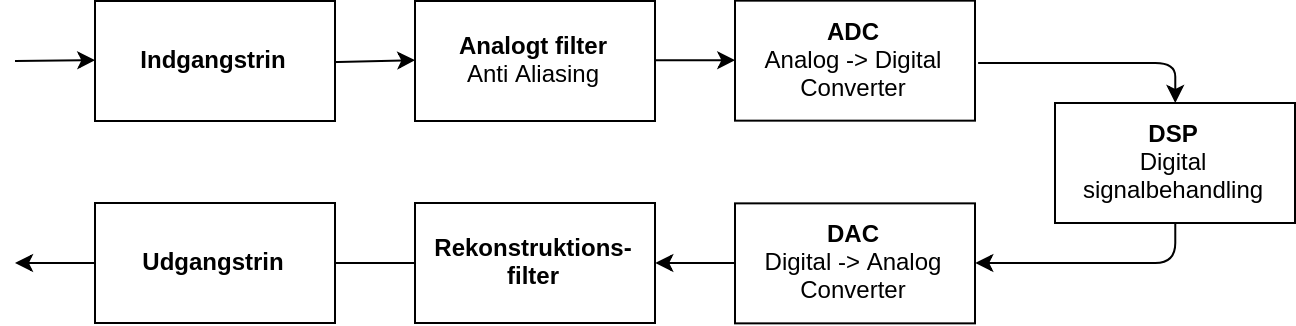
\includegraphics[width=.9\textwidth]{billeder/model.png}
	\caption{Løsningsmodel som blokdiagram}
	\label{fig:model}
\end{figure}

Modellen indeholder de mest basale blokke der er nødvendige for at opnå en løsning og signalet følger pilenes retning.

Modellens enkelte blokke danner grundlag for denne rapports opbygning og vil blive gennemgået og gennemarbejdet i de efterfølgende kapitler.


\section{Implementerings trin}

\subsection{Trin 1}
Implementering af anti aliasing filtrene som diskrete bi-quad moduler. 
Derved kan det enkelte moduls virkemåde eftervises og chancen for konstruktionsfejl nedsættes.
Simpelt styresystem implementeres med et basis udvalg af effekter.

\subsection{Trin 2}
\textit{Planlagt trin, men ikke opnået indenfor projektets tidsramme.}
\\
\\
Den samlede løsning sammenbygges til én enhed og effektiviseres med hensyn til bl.a. komponent valg. 
Andre faktorer som fx over- eller underdimensionering af krav til løsning kan også tilpasses her, så en mere fornuftig og anvendelig løsning opnås.
Et mere generisk styresystem implementeres og muligheden for equalizer filtre tilføjes, som fx lavpas, højpas og andre profiler. 
